\documentclass{article}
\usepackage{lipsum}
\usepackage{geometry}
\usepackage{amsmath}
\usepackage{graphicx}
\linespread{1.5}
\author{Sergio Garcia-Rios 
	\thanks{Cornell University - Government}
	}
\title{Anxiously Preparing for a Final Paper: \\ 
A \LaTeX\  Template for ARA Students}
\date{}




\begin{document}

\maketitle
\clearpage

\section{Introduction}
\lipsum[1-3]

\section{Theory and Hypotheses}
\lipsum[2]

% Comment here
\subsection{Hypotheses}
\lipsum[2] This here \footnote{This is the footnote stuff} is a footnote

\begin{itemize}
    \item Hypothesis 1: Lorem ipsum dolor sit amet, consectetuer adipiscing elit. Aenean commodo
    \item Hypothesis 2 Sed ut perspiciatis unde omnis iste natus error sit voluptatem accusantium doloremque
\end{itemize}


\lipsum[1]

\section{Data and Methods}

\lipsum[2]


\begin{table}[!htbp] \centering 
  \caption{Descriptive Statistics for Variables Used} 
  \label{tab: desc} 
\begin{tabular}{@{\extracolsep{5pt}}lccccccc} 
\\[-1.8ex]\hline 
\hline \\[-1.8ex] 
Statistic & \multicolumn{1}{c}{N} & \multicolumn{1}{c}{Mean} & \multicolumn{1}{c}{St. Dev.} & \multicolumn{1}{c}{Min} & \multicolumn{1}{c}{Pctl(25)} & \multicolumn{1}{c}{Pctl(75)} & \multicolumn{1}{c}{Max} \\ 
\hline \\[-1.8ex] 
Vote for Trump & 3,368 & 0.403 & 0.491 & 0.000 & 0.000 & 1.000 & 1.000 \\ 
Male & 4,219 & 0.471 & 0.499 & 0.000 & 0.000 & 1.000 & 1.000 \\ 
Income & 4,069 & 15.387 & 8.080 & 1.000 & 9.000 & 22.000 & 28.000 \\ 
Age & 4,150 & 49.576 & 17.581 & 18.000 & 34.000 & 63.000 & 90.000 \\ 
Conservative & 4,191 & 4.171 & 1.453 & 1.000 & 3.000 & 5.000 & 7.000 \\ 
Education & 4,227 & 11.171 & 2.325 & 1.000 & 9.000 & 13.000 & 16.000 \\ 
Sexism & 4,154 & 2.675 & 1.165 & 1.000 & 2.000 & 3.000 & 5.000 \\ 
Oppose Aff Action & 4,224 & 2.261 & 0.750 & 1.000 & 2.000 & 3.000 & 3.000 \\ 
Immigration Axiety & 3,622 & 3.473 & 1.139 & 1.000 & 3.000 & 4.750 & 5.000 \\ 
Economic Anxiety & 3,639 & 3.031 & 1.017 & 1.000 & 2.000 & 4.000 & 5.000 \\ 
White & 4,211 & 0.810 & 0.392 & 0.000 & 1.000 & 1.000 & 1.000 \\ 
\hline \\[-1.8ex] 
\end{tabular} 
\end{table} 

\lipsum[3]

\subsection{Models and specification}

\lipsum[4]


\begin{multline}
  \operatorname{Pr}(\text{Vote} = 1 \mid \text{H, T})\\
 = \frac{\exp(\beta_{0} + \beta_{1} \text{Gender} + \beta_{2} \text{Age} + \dots +
    \beta_{12} \text{immigration)} }{1 + \exp(\beta_{0} + \beta_{1} \text{Gender} + \beta_{2} \text{Age} +
\dots + \beta_{12 }\text{immigration})} \label{eq:glm1} 
\end{multline}



\lipsum[5]



\section{Results}

\lipsum[2]

I can reference Table \ref{tab: regs} here and can reference Figure \ref{fig: ame} and Equation \ref{eq:glm1}



\begin{table}[!htbp] \centering 
  \caption{Logistic Regression: Trump something something} 
  \label{tab: regs} 
\begin{tabular}{@{\extracolsep{5pt}}lccc} 
\\[-1.8ex]\hline 
\hline \\[-1.8ex] 
 & \multicolumn{3}{c}{\textit{Dependent variable:}} \\ 
\cline{2-4} 
\\[-1.8ex] & \multicolumn{3}{c}{Vote for Trump} \\ 
\\[-1.8ex] & (1) & (2) & (3)\\ 
\hline \\[-1.8ex] 
 Male & 0.077 (0.099) & 0.069 (0.107) & 0.134 (0.119) \\ 
  Income & 0.001 (0.007) & 0.0003 (0.008) & $-$0.001 (0.008) \\ 
  Age & 0.005$^{*}$ (0.003) & 0.007$^{**}$ (0.003) & 0.001 (0.003) \\ 
  Conservative & 1.192$^{***}$ (0.046) & 1.200$^{***}$ (0.050) & 1.061$^{***}$ (0.056) \\ 
  Education & $-$0.096$^{***}$ (0.024) & $-$0.092$^{***}$ (0.026) & $-$0.038 (0.029) \\ 
  Sexism &  &  & 0.275$^{***}$ (0.054) \\ 
  Oppose Aff Action &  &  & 0.546$^{***}$ (0.088) \\ 
  Immigration Axiety &  &  & 0.793$^{***}$ (0.060) \\ 
  Economic Anxiety &  & 0.091$^{*}$ (0.053) & $-$0.049 (0.059) \\ 
  White & 2.225$^{***}$ (0.170) & 2.130$^{***}$ (0.184) & 1.920$^{***}$ (0.199) \\ 
  Constant & $-$6.748$^{***}$ (0.377) & $-$7.104$^{***}$ (0.474) & $-$11.171$^{***}$ (0.619) \\ 
 \hline \\[-1.8ex] 
Observations & 3,082 & 2,667 & 2,625 \\ 
Log Likelihood & $-$1,297.942 & $-$1,119.679 & $-$950.481 \\ 
Akaike Inf. Crit. & 2,609.884 & 2,255.357 & 1,922.962 \\ 
\hline 
\hline \\[-1.8ex] 
\textit{Note:}  & \multicolumn{3}{r}{$^{*}$p$<$0.1; $^{**}$p$<$0.05; $^{***}$p$<$0.01} \\ 
\end{tabular} 
\end{table} 


\lipsum[5-6]


\begin{figure}
\centering
\caption{This is the title for this figure}
\label{fig: ame}
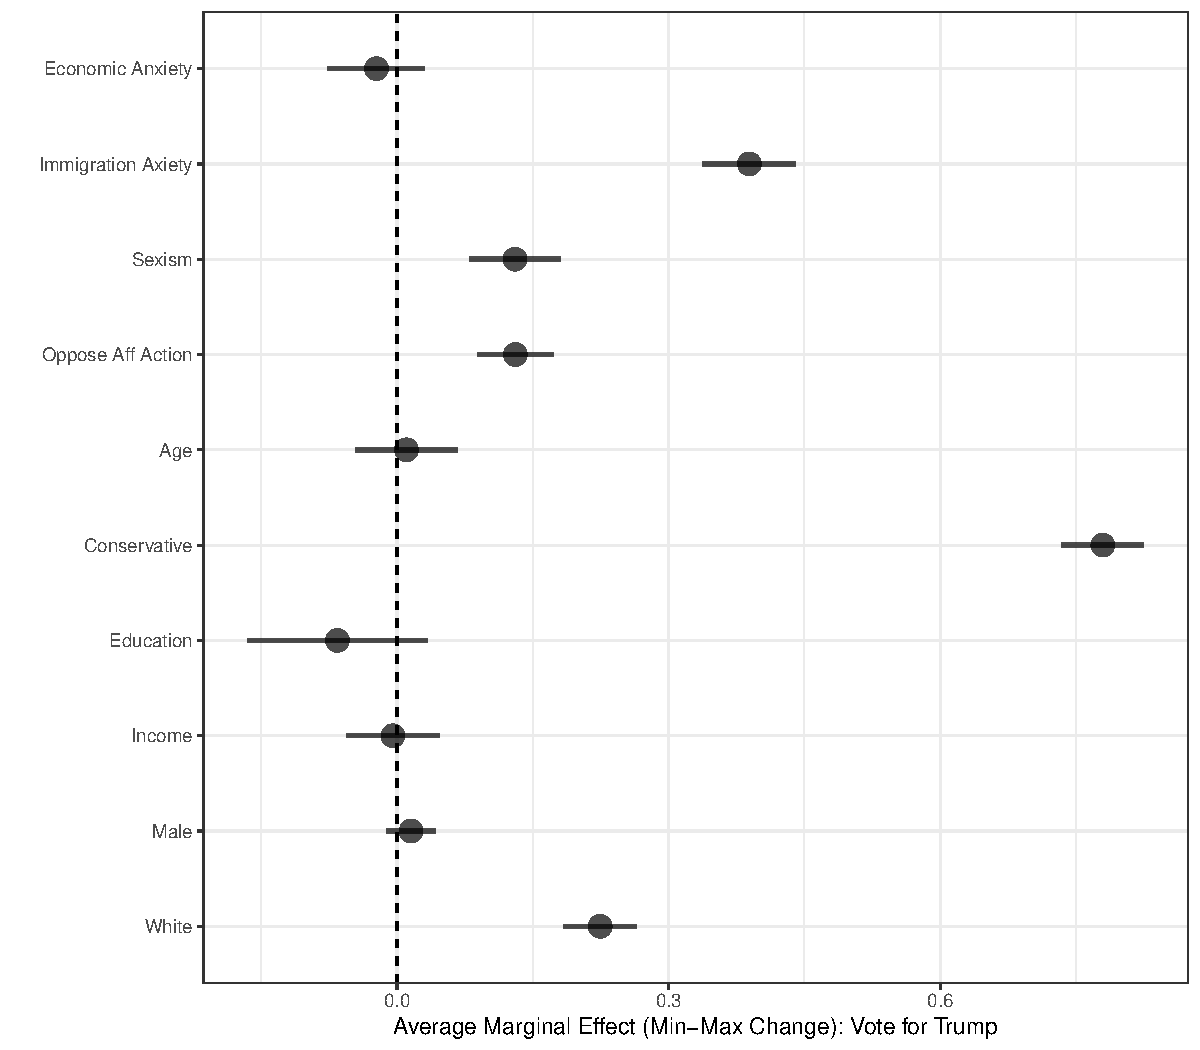
\includegraphics[scale=.6]{ame_plot}
\end{figure}

\lipsum[5]


\begin{figure}
\centering
\caption{This is the title for this figure}
\label{fig: preds}
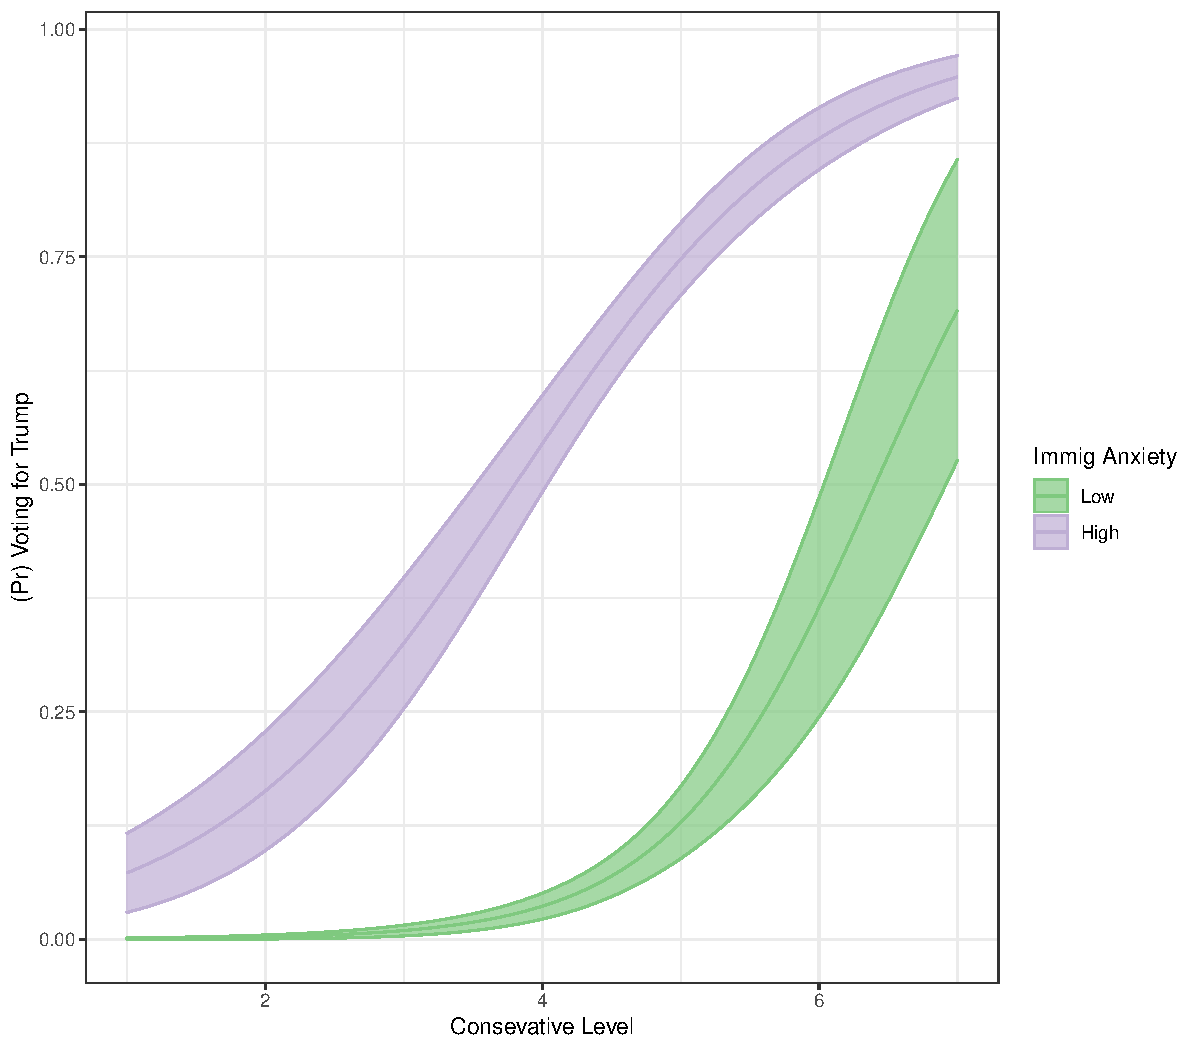
\includegraphics[scale=.6]{preds}
\end{figure}

\lipsum[8]

\section{Conclusion}

\lipsum[20-22]




\end{document}


































































